\chapter{Assignment: Considerations, Notations, Strategy}
This appendix presents several strategies and tools for understanding and 
applying the concepts of resonances and GSSs during chemical shift assignment.
These were all developed during the course of analysis of the Samp3 data set,
and were concurrently applied in order to facilitate correct analysis.


\section{Typing of H-N-rooted GSSs}
Type assignment of GSSs is an important intermediate for obtaining 
sequence-specific GSS assignments.  There are several categories of H-N-rooted
GSSs.  Backbone GSSs are rooted in the H-N of the peptide backbone.  Sidechain 
GSSs are rooted in H-N groups of amino acid sidechains.
The backbone ones may span multiple amino acid residues; the typing of the 
corresponding residues may be known partially or fully for each piece.

A simple system is presented in Figure \ref{hn_gss_types} for representing 
partial and full GSS typing.  First, the typing of a portion of a GSS may be 
ambiguous or unambiguous.  If it is unambiguous, then a single type is assigned
to that portion.  If it is ambiguous, then multiple types are assigned to that
portion.  An ambiguous assignment may be one of several, such as either a
Serine or a Threonine; it may be one of many, such as any backbone type; or
it may be any H-N-rooted GSS type.  A sequential assignment, which only applies
to backbone GSSs as they are able to span multiple amino acids, enables 
independent typing of each amino acid spanned by the GSS.


\section{Graph patterns of pulse sequences}
Modeling pulse sequences as patterns which act upon graphs is simplistic but
useful.  The graphs are molecules, the nodes are nuclei, and scalar and
dipolar couplings are edges.  Wherever a pulse sequence pattern matches 
a molecular graph, signals are expected in the corresponding spectra.

The model separates nuclei into groups based on atomic number
and chemical shift range, yielding protons, nitrogens, aliphatic Carbon,
aromatic Carbon, and carbonyl Carbon (see Table \ref{pulse_sequence_key}).
Nuclei are connected by J-couplings or through-space couplings, 
indicating transfer of magnetization between nuclei.
Finally, a differentiation is made between nuclei whose chemical shift is 
and is not recorded.  See Tables \ref{pulse_sequence_key} and 
\ref{pulse_sequence_patterns}.

This approach is similar to that applied in \cite{fox2004delineation}; a major
difference is that NMR-specific details such as specific J-coupling values, 
decoupling pulses, shaped pulses, and transfer efficiencies have all been 
omitted.  These were omitted in order to keep the model simple and easy to use,
so that it is possible to quickly determine which atoms and spin systems are 
expected in an NMR experiment.


\section{Partial ambiguities in resonance typing}
Resonance typing interacts with GSS typing, as the GSS type(s) determine
which atoms may possibly be present in a GSS, and which atoms a pulse 
sequence can observe.  However, it is still possible to obtain partial 
resonance typings -- depending on the pulse sequences used -- without
unambiguously typing the containing GSS.  Two cases where such information
is obtainable are an HNCACB, which distinguishes between the "CA" and "CB"
atoms by means of a 180-degree phase shift, and experiment pairs such as the
HNCACB and HN(CO)CACB, which allows for distinguishing between CA and CA(i-1),
and CB and CB(i-1) based on peaks which do and do not appear at the same 
chemical shift in both spectra.
Figures 
\ref{generic_hncacb},
\ref{generic_hncacb_ambiguous},
\ref{backbone_hncacb_ambiguous},
\ref{sidechain_qn_hncacb},
\ref{sidechain_q_hncacb} and
\ref{sidechain_r_hncacb}
present a scheme for capturing these partial resonance typings based on the
key given in Table \ref{partial_typing_notation}.


\clearpage
\section{Tables}

\begin{table}[h]
    \begin{tabular}{ | c | c | }
    \hline
      GSS typing            &   Shorthand notation    \\ \hline
      \hline
      Unknown               &   ?                     \\ \hline
      Single backbone       &   A,C,D,E,F,G,H,I,K,L,M,N,Q,R,S,T,V,W,Y   \\ \hline
      Single backbone (i-1) &   A,C,D,E,F,G,H,I,K,L,M,N,P,Q,R,S,T,V,W,Y   \\ \hline
      Ambiguous backbone    &   b                     \\ \hline
      Single sidechain      &   sQ, sN, sW, sR        \\ \hline
      Backbone S/T          &   S/T                   \\ \hline
      Sidechain Q/N         &   sQ/sN                 \\ \hline
      Sequential            &   b-b, I-S, P/R-G       \\ \hline
    \end{tabular}
    \caption[GSS types used in typing of H-N-rooted GSSs.]
            {GSS types used in typing of H-N-rooted GSSs.  In addition to the
             basic GSS types from standard H-N groups present in protein
             backbones and amino acid sidechains,
             fully and partially ambiguous GSS types are useful.  GSSs that
             span multiple amino acids are given a separate type for each
             amino acid.}
    \label{hn_gss_types}
\end{table}

\begin{table}
    \begin{tabular}{ | c | c | }
      \hline
      Symbol    &  Explanation              \\  \hline
      \hline
      Hn        &  Any H                    \\  \hline
      Nn        &  Any N                    \\  \hline
      Ca        &  Aliphatic C              \\  \hline
      Co        &  Carbonyl C               \\  \hline
      Cr        &  Aromatic C               \\  \hline
      --        &  J-coupling               \\  \hline
      <-->      &  Through-space coupling   \\  \hline
      [...]     &  Chemical shift not collected  \\  \hline
      ...*      &  Zero or more             \\  \hline
      ...+      &  One or more              \\  \hline
    \end{tabular}
    \caption[Key used to model various common pulse sequences as patterns on graphs.]
            {Key used to model various common pulse sequences as patterns
             on graphs.  Nuclei form the nodes of the graph, and J-couplings
             form the edges.}
    \label{pulse_sequence_key}
\end{table}

\begin{table}
    \begin{tabular}{ | c | c | }
    \hline
    NHSQC           &  Hn -- Nn                                \\  \hline
    HNCO            &  Hn -- Nn -- Co                          \\  \hline
    HN(CA)CO        &  Hn -- Nn -- [Ca] -- Co                  \\  \hline
    HNCA            &  Hn -- Nn -- Ca                          \\  \hline
    HNCACB          &  Hn -- Nn -- Ca1                         \\  \hline
    HNCACB          &  Hn -- Nn -- [Ca1] -- Ca2                \\  \hline
    HN(CO)CACB      &  Hn -- Nn -- [Co] -- Ca1                 \\  \hline
    HN(CO)CACB      &  Hn -- Nn -- [Co] -- [Ca1] -- Ca2        \\  \hline
    C(CO)NH-TOCSY   &  Hn -- Nn -- [Co] -- [Ca]* -- Ca         \\  \hline
    H(CCO)NH-TOCSY  &  Hn -- Nn -- [Co] -- [Ca]+ -- Hn         \\  \hline
    HBHA(CO)NH      &  Hn -- Nn -- [Co] -- [Ca] -- Hn          \\  \hline
    HBHA(CO)NH      &  Hn -- Nn -- [Co] -- [Ca] -- [Ca] -- Hn  \\  \hline
    HCCH-TOCSY      &  Hn -- Ca -- [Ca]* -- Hn                 \\  \hline
    TOCSY-NHSQC     &  Hn -- Nn -- [Ca]+ -- Hn                 \\  \hline
    hbCBcgcdHD      &  [Hn] -- Ca -- [Cr]{2} -- Hn             \\  \hline
    hbCBcgcdceHE    &  [Hn] -- Ca -- [Cr]{2,3} -- Hn           \\  \hline  
    CHSQC           &  Hn -- C                                 \\  \hline
    NOESY-NHSQC     &  Hn <--> Hn -- Nn                        \\  \hline
    NOESY-CHSQC     &  Hn <--> Hn -- C                         \\  \hline
    \end{tabular}
    \caption{Common pulse sequences and their graph patterns using the key
             given in Table \ref{pulse_sequence_key}.}
    \label{pulse_sequence_patterns}
\end{table}

\begin{table}
  \begin{tabular}{ | c | c | c |}
    \hline
    Atoms       &  Together &  Separate      \\  \hline 
    HA2/HA3     &  HA*      &  HA*1, HA*2    \\  \hline 
    HB2/HB3     &  HB*      &  HB*1, HB*2    \\  \hline 
    HE21/HE22   &  HE2*     &  HE2*1, HE2*2  \\  \hline 
    QG1/QG2     &  QG*      &  QG*1, QG*2    \\  \hline
    Ca11/Ca12   &  Ca1*     &  Ca1*1, Ca1*2  \\  \hline
    Ca11/Ca21   &  Ca*1     &  Ca*11, Ca*21  \\  \hline
  \end{tabular}
  \caption[Notation for partial resonance typings.]
          {Notation for partial resonance typings.
           In general, each group includes multiple nuclei which may be 
           ambiguous depending on the pulse sequences used and the 
           state of the assignment of the full data set.
           For stereospecially ambiguous atoms, the names are formed by
           replacing the number with a * to signify all atoms, and appending
           a unique index to signify one but not all of the atoms.}
  \label{partial_typing_notation}
\end{table}


\clearpage
\section{Figures}

\begin{figure}[h]
  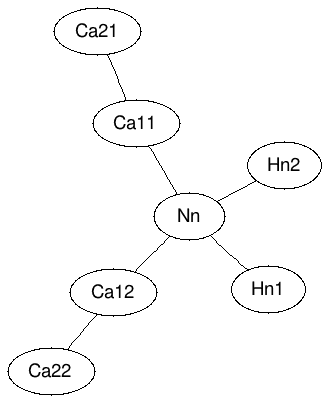
\includegraphics[scale=0.75]{figures/generic_hncacb}
  \caption[The portion of a GSS observable from an HNCACB experiment.]
          {The portion of a GSS observable from an HNCACB experiment.
           The atom names reflect their relationships: Ca11 and Ca21 are
           distinguishable from Ca12 and Ca22 by a 180-degree phase shift,
           while Ca11 and Ca12 form a distinct covalent group from Ca21 and Ca22.}
  \label{generic_hncacb}
\end{figure}    

\begin{figure}
  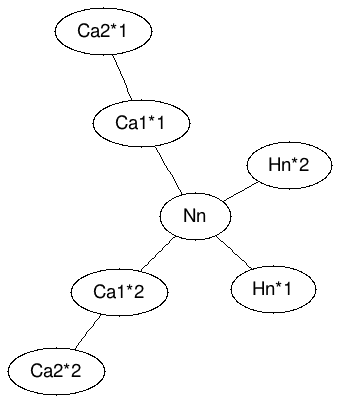
\includegraphics[scale=0.75]{figures/generic_hncacb_ambiguous}
  \caption[An alternative naming scheme which accounts for ambiguity.]
          {An alternative naming scheme which accounts for ambiguity for
           GSSs observed through an HNCACB.  Distinct, placeholder names are
           used to indicate the important relationships between resonances:
           the number of bonds distance of the aliphatic Carbons from the
           Nitrogen.}
  \label{generic_hncacb_ambiguous}
\end{figure}

\begin{figure}
  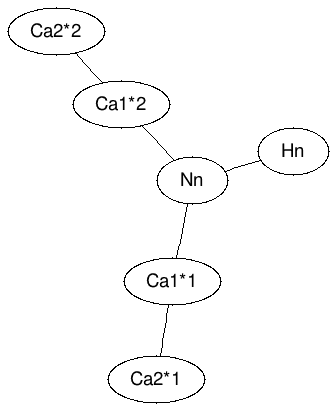
\includegraphics[scale=0.75]{figures/backbone_hncacb_ambiguous}
  \caption[A backbone GSS in HNCACB.]
          {A backbone GSS in HNCACB.  Note that 
           the Ca11/Ca21 and Ca12/Ca22 pairs may be ambiguous.}
  \label{backbone_hncacb_ambiguous}
\end{figure}

\begin{figure}
  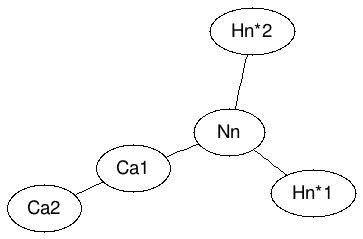
\includegraphics[scale=0.75]{figures/sidechain_qn_hncacb}
  \caption[The extent of a sidechain Q or N GSS in an HNCACB.]
          {The extent of a sidechain Q or N GSS in an HNCACB.  Note that
           there are two protons, which may be ambiguously assigned.}
  \label{sidechain_qn_hncacb}
\end{figure}

\begin{figure}
  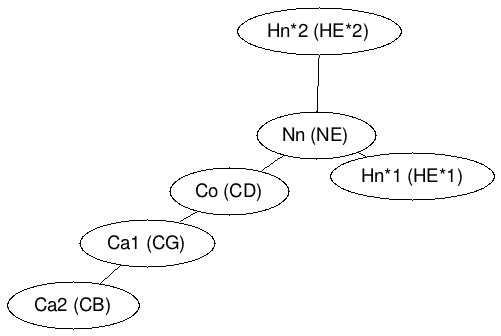
\includegraphics[scale=0.75]{figures/sidechain_q_hncacb}
  \caption[A GSS in an HNCACB, assigned to a Q sidechain.]
          {A GSS in an HNCACB, assigned to a Q sidechain.
           The nitrogen and carbon resonances have been unambiguously
           typed, while the proton resonances are ambiguous.}
  \label{sidechain_q_hncacb}
\end{figure}

\begin{figure}
  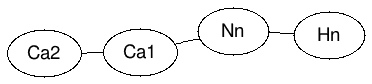
\includegraphics[scale=0.75]{figures/sidechain_r_hncacb}
  \caption[A sidechain R gss in an HNCACB].
          {A sidechain R GSS in an HNCACB.  The resonances have not
           yet been typed.}
  \label{sidechain_r_hncacb}
\end{figure}

